% Options for packages loaded elsewhere
\PassOptionsToPackage{unicode}{hyperref}
\PassOptionsToPackage{hyphens}{url}
\PassOptionsToPackage{dvipsnames,svgnames,x11names}{xcolor}
%
\documentclass[
  letterpaper,
  DIV=11,
  numbers=noendperiod]{scrartcl}

\usepackage{amsmath,amssymb}
\usepackage{iftex}
\ifPDFTeX
  \usepackage[T1]{fontenc}
  \usepackage[utf8]{inputenc}
  \usepackage{textcomp} % provide euro and other symbols
\else % if luatex or xetex
  \usepackage{unicode-math}
  \defaultfontfeatures{Scale=MatchLowercase}
  \defaultfontfeatures[\rmfamily]{Ligatures=TeX,Scale=1}
\fi
\usepackage{lmodern}
\ifPDFTeX\else  
    % xetex/luatex font selection
\fi
% Use upquote if available, for straight quotes in verbatim environments
\IfFileExists{upquote.sty}{\usepackage{upquote}}{}
\IfFileExists{microtype.sty}{% use microtype if available
  \usepackage[]{microtype}
  \UseMicrotypeSet[protrusion]{basicmath} % disable protrusion for tt fonts
}{}
\makeatletter
\@ifundefined{KOMAClassName}{% if non-KOMA class
  \IfFileExists{parskip.sty}{%
    \usepackage{parskip}
  }{% else
    \setlength{\parindent}{0pt}
    \setlength{\parskip}{6pt plus 2pt minus 1pt}}
}{% if KOMA class
  \KOMAoptions{parskip=half}}
\makeatother
\usepackage{xcolor}
\setlength{\emergencystretch}{3em} % prevent overfull lines
\setcounter{secnumdepth}{5}
% Make \paragraph and \subparagraph free-standing
\makeatletter
\ifx\paragraph\undefined\else
  \let\oldparagraph\paragraph
  \renewcommand{\paragraph}{
    \@ifstar
      \xxxParagraphStar
      \xxxParagraphNoStar
  }
  \newcommand{\xxxParagraphStar}[1]{\oldparagraph*{#1}\mbox{}}
  \newcommand{\xxxParagraphNoStar}[1]{\oldparagraph{#1}\mbox{}}
\fi
\ifx\subparagraph\undefined\else
  \let\oldsubparagraph\subparagraph
  \renewcommand{\subparagraph}{
    \@ifstar
      \xxxSubParagraphStar
      \xxxSubParagraphNoStar
  }
  \newcommand{\xxxSubParagraphStar}[1]{\oldsubparagraph*{#1}\mbox{}}
  \newcommand{\xxxSubParagraphNoStar}[1]{\oldsubparagraph{#1}\mbox{}}
\fi
\makeatother


\providecommand{\tightlist}{%
  \setlength{\itemsep}{0pt}\setlength{\parskip}{0pt}}\usepackage{longtable,booktabs,array}
\usepackage{calc} % for calculating minipage widths
% Correct order of tables after \paragraph or \subparagraph
\usepackage{etoolbox}
\makeatletter
\patchcmd\longtable{\par}{\if@noskipsec\mbox{}\fi\par}{}{}
\makeatother
% Allow footnotes in longtable head/foot
\IfFileExists{footnotehyper.sty}{\usepackage{footnotehyper}}{\usepackage{footnote}}
\makesavenoteenv{longtable}
\usepackage{graphicx}
\makeatletter
\def\maxwidth{\ifdim\Gin@nat@width>\linewidth\linewidth\else\Gin@nat@width\fi}
\def\maxheight{\ifdim\Gin@nat@height>\textheight\textheight\else\Gin@nat@height\fi}
\makeatother
% Scale images if necessary, so that they will not overflow the page
% margins by default, and it is still possible to overwrite the defaults
% using explicit options in \includegraphics[width, height, ...]{}
\setkeys{Gin}{width=\maxwidth,height=\maxheight,keepaspectratio}
% Set default figure placement to htbp
\makeatletter
\def\fps@figure{htbp}
\makeatother
% definitions for citeproc citations
\NewDocumentCommand\citeproctext{}{}
\NewDocumentCommand\citeproc{mm}{%
  \begingroup\def\citeproctext{#2}\cite{#1}\endgroup}
\makeatletter
 % allow citations to break across lines
 \let\@cite@ofmt\@firstofone
 % avoid brackets around text for \cite:
 \def\@biblabel#1{}
 \def\@cite#1#2{{#1\if@tempswa , #2\fi}}
\makeatother
\newlength{\cslhangindent}
\setlength{\cslhangindent}{1.5em}
\newlength{\csllabelwidth}
\setlength{\csllabelwidth}{3em}
\newenvironment{CSLReferences}[2] % #1 hanging-indent, #2 entry-spacing
 {\begin{list}{}{%
  \setlength{\itemindent}{0pt}
  \setlength{\leftmargin}{0pt}
  \setlength{\parsep}{0pt}
  % turn on hanging indent if param 1 is 1
  \ifodd #1
   \setlength{\leftmargin}{\cslhangindent}
   \setlength{\itemindent}{-1\cslhangindent}
  \fi
  % set entry spacing
  \setlength{\itemsep}{#2\baselineskip}}}
 {\end{list}}
\usepackage{calc}
\newcommand{\CSLBlock}[1]{\hfill\break\parbox[t]{\linewidth}{\strut\ignorespaces#1\strut}}
\newcommand{\CSLLeftMargin}[1]{\parbox[t]{\csllabelwidth}{\strut#1\strut}}
\newcommand{\CSLRightInline}[1]{\parbox[t]{\linewidth - \csllabelwidth}{\strut#1\strut}}
\newcommand{\CSLIndent}[1]{\hspace{\cslhangindent}#1}

\KOMAoption{captions}{tableheading}
\makeatletter
\@ifpackageloaded{caption}{}{\usepackage{caption}}
\AtBeginDocument{%
\ifdefined\contentsname
  \renewcommand*\contentsname{Table of contents}
\else
  \newcommand\contentsname{Table of contents}
\fi
\ifdefined\listfigurename
  \renewcommand*\listfigurename{List of Figures}
\else
  \newcommand\listfigurename{List of Figures}
\fi
\ifdefined\listtablename
  \renewcommand*\listtablename{List of Tables}
\else
  \newcommand\listtablename{List of Tables}
\fi
\ifdefined\figurename
  \renewcommand*\figurename{Figure}
\else
  \newcommand\figurename{Figure}
\fi
\ifdefined\tablename
  \renewcommand*\tablename{Table}
\else
  \newcommand\tablename{Table}
\fi
}
\@ifpackageloaded{float}{}{\usepackage{float}}
\floatstyle{ruled}
\@ifundefined{c@chapter}{\newfloat{codelisting}{h}{lop}}{\newfloat{codelisting}{h}{lop}[chapter]}
\floatname{codelisting}{Listing}
\newcommand*\listoflistings{\listof{codelisting}{List of Listings}}
\makeatother
\makeatletter
\makeatother
\makeatletter
\@ifpackageloaded{caption}{}{\usepackage{caption}}
\@ifpackageloaded{subcaption}{}{\usepackage{subcaption}}
\makeatother

\ifLuaTeX
  \usepackage{selnolig}  % disable illegal ligatures
\fi
\usepackage{bookmark}

\IfFileExists{xurl.sty}{\usepackage{xurl}}{} % add URL line breaks if available
\urlstyle{same} % disable monospaced font for URLs
\hypersetup{
  pdftitle={My title},
  pdfauthor={First author; Another author},
  colorlinks=true,
  linkcolor={blue},
  filecolor={Maroon},
  citecolor={Blue},
  urlcolor={Blue},
  pdfcreator={LaTeX via pandoc}}


\title{My title\thanks{Code and data are available at:
\url{https://github.com/RohanAlexander/starter_folder}.}}
\usepackage{etoolbox}
\makeatletter
\providecommand{\subtitle}[1]{% add subtitle to \maketitle
  \apptocmd{\@title}{\par {\large #1 \par}}{}{}
}
\makeatother
\subtitle{My subtitle if needed}
\author{First author \and Another author}
\date{November 2, 2024}

\begin{document}
\maketitle
\begin{abstract}
First sentence. Second sentence. Third sentence. Fourth sentence.
\end{abstract}


\section{Introduction}\label{introduction}

Overview paragraph

Estimand paragraph

Results paragraph

Why it matters paragraph

Telegraphing paragraph: The remainder of this paper is structured as
follows. Section~\ref{sec-data}\ldots.

\section{Data}\label{sec-data}

\subsection{Overview}\label{overview}

In this analysis, we used R (R Core Team 2023) to investigate polling
data on public sentiment leading up to the election. Our dataset,
sourced from FiveThirtyEight (FiveThirtyEight 2024), provides a detailed
snapshot of shifting public opinion over time. We examined key factors
influencing support percentages, including poll timing, pollster
characteristics, and state-specific trends.

Several R packages were instrumental in facilitating data manipulation,
modeling, and visualization. Tidyverse served as the foundation for
organizing and efficiently analyzing the data, seamlessly integrating
multiple analytical tasks (Wickham et al. 2019). The Here package
simplified file path management, ensuring smooth data access across
systems (\textbf{citehere?}). We utilized Janitor for comprehensive data
cleaning, which helped us identify and correct inconsistencies
(\textbf{citejanitor?}), while Lubridate supported the handling of
time-related variables (\textbf{citelubridate?}). Finally, Arrow enabled
fast, memory-efficient access to large datasets, a crucial asset when
working with extensive polling data (\textbf{citearrow?}). Our codebase
and workflow adhered closely to best practices, as outlined in Alexander
(2023).

Our group focused on Trump's approval ratings, aiming to ensure the
credibility of the data. To achieve this, we selected only pollsters
with ratings above 2, using data collected from November 15, 2022, to
October 27, 2024. Overview text

\subsection{Measurement}\label{measurement}

The data comes from FiveThirtyEight, where we look primarily at Trump's
electoral margins

\subsection{Outcome variables}\label{outcome-variables}

\subsubsection{Overview of Trump's Electoral
Support}\label{overview-of-trumps-electoral-support}

Figure~\ref{fig-pct} illustrates the distribution of approval ratings
for Trump. The majority of the approval ratings fall between 40\% and
55\%, forming a shape that resembles a normal distribution, with a peak
around the 45\% to 50\% range. This suggests that, within the analyzed
sample, most of the approval ratings cluster in this middle range, with
relatively few instances of extremely high or low ratings.

The lower frequency of approval ratings below 30\% and above 60\%
indicates that these extremes are relatively uncommon in the dataset.
Overall, the concentration of support in this central range suggests a
fairly consistent level of public support for Trump.

\begin{figure}

\centering{

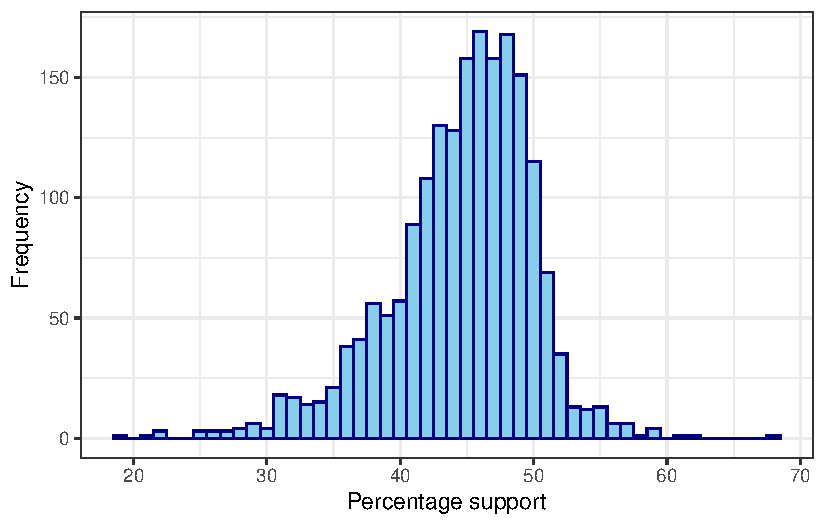
\includegraphics{paper_files/figure-pdf/fig-pct-1.pdf}

}

\caption{\label{fig-pct}Distribution of percentage support for Trump}

\end{figure}%

\subsubsection{Overview of election data in different
states}\label{overview-of-election-data-in-different-states}

Here we looked at how each state polled in the popular vote. What we
found for each state had to do with its party affiliation. the REP
partisan states would have a higher Trump vote, above 50 per cent. then
there are the swing states where the number of votes generally swings
around the 50 mark. And states that are predominantly DEM partisan will
have much lower support for Trump generally below 50 per cent

\begin{figure}

\centering{

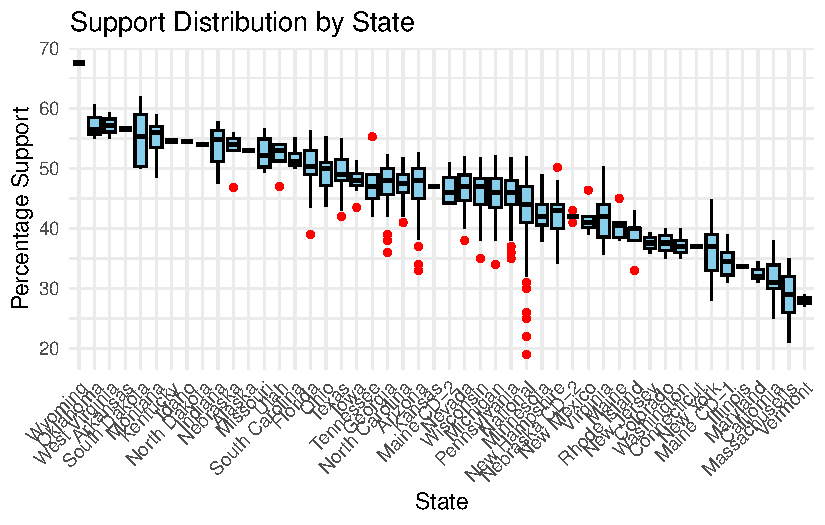
\includegraphics{paper_files/figure-pdf/fig-state-1.pdf}

}

\caption{\label{fig-state}state and poll}

\end{figure}%

\subsubsection{Overview of voting
method}\label{overview-of-voting-method}

The primary data collection methods include online panels, live phone
interviews, automated phone surveys, and mail questionnaires. These
methods are widely used due to their efficiency in reaching diverse
respondent groups. Online panels are suitable for internet users, live
phone interviews allow for detailed feedback and access to those less
active online, automated phone surveys are cost-effective with broad
reach, and mail questionnaires are ideal for older individuals or those
not using the internet. The variety of these methods ensures broad
representation and accuracy in the data.

\begin{figure}

\centering{

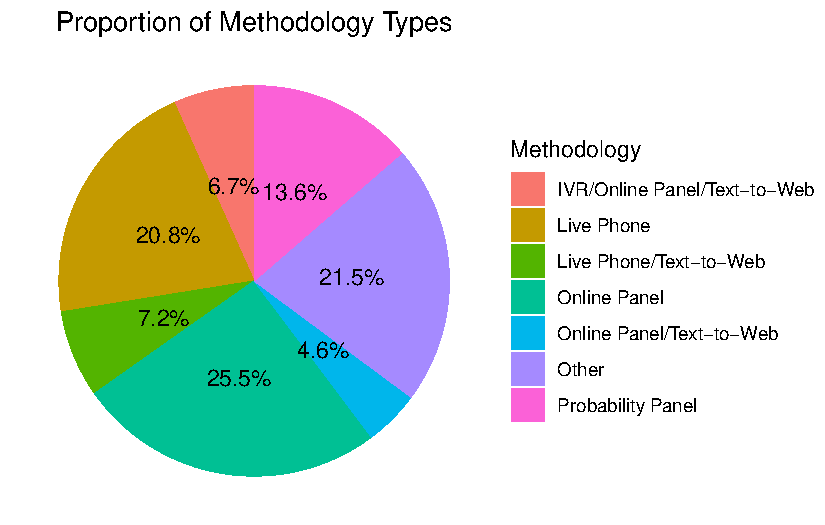
\includegraphics{paper_files/figure-pdf/fig-method-1.pdf}

}

\caption{\label{fig-method}method}

\end{figure}%

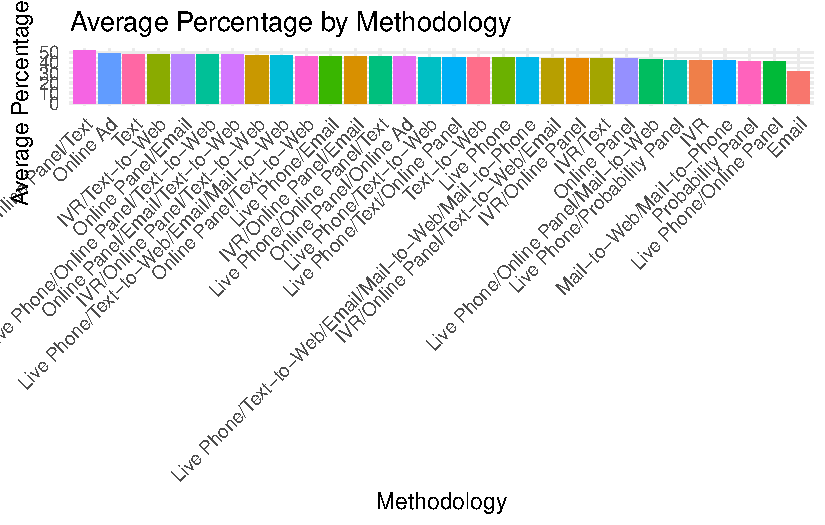
\includegraphics{paper_files/figure-pdf/fig-method&pct-1.pdf}\{\#fig-method\&pct\}

\subsection{Predictor variables}\label{predictor-variables}

Add graphs, tables and text.

Use sub-sub-headings for each outcome variable and feel free to combine
a few into one if they go together naturally.

\phantomsection\label{refs}
\begin{CSLReferences}{1}{0}
\bibitem[\citeproctext]{ref-tellingstories}
Alexander, Rohan. 2023. \emph{Telling Stories with Data}. Chapman;
Hall/CRC. \url{https://tellingstorieswithdata.com/}.

\bibitem[\citeproctext]{ref-fivethirtyeight2024}
FiveThirtyEight. 2024. {``Dataset: US Presidential General Election
Polls.''}
\url{https://projects.fivethirtyeight.com/polls/data/president_polls.csv}.

\bibitem[\citeproctext]{ref-citeR}
R Core Team. 2023. \emph{{R: A Language and Environment for Statistical
Computing}}. Vienna, Austria: R Foundation for Statistical Computing.
\url{https://www.R-project.org/}.

\bibitem[\citeproctext]{ref-thereferencecanbewhatever}
Wickham, Hadley, Mara Averick, Jennifer Bryan, Winston Chang, Lucy
D'Agostino McGowan, Romain François, Garrett Grolemund, et al. 2019.
{``Welcome to the {tidyverse}.''} \emph{Journal of Open Source Software}
4 (43): 1686. \url{https://doi.org/10.21105/joss.01686}.

\end{CSLReferences}




\end{document}
